\section{AWStream: Network Resource Adaptation}

\begin{frame}{Scarce and Variable Bandwidth}

\end{frame}

\begin{frame}{Fidelity vs.\,Freshness}
  \vspace{2em}
  \begin{figure}
    \centering
    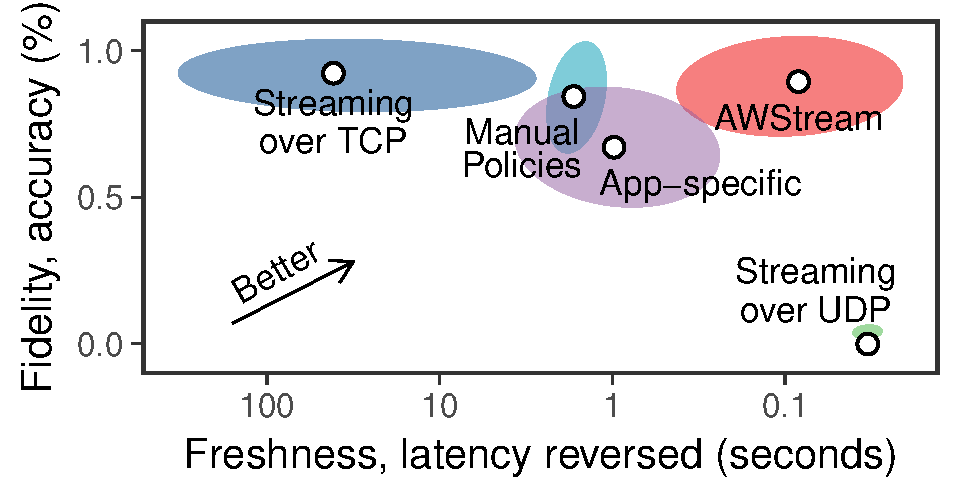
\includegraphics[width=0.8\columnwidth]{figures/fidelity-freshness.pdf}
    \caption{The trade-off space between data freshness and fidelity when facing
      insufficient bandwidth.}
  \end{figure}
\end{frame}

\captionsetup[figure]{labelformat=empty,font=scriptsize,labelfont=scriptsize}
\begin{frame}{Application-specific Optimizations Don't Generalize}
  \pgfplotstableread[row sep=\\,col sep=&]{
    Frame Rate & Bandwidth (normalized) & Accuracy \\
    30 & 100 & 100 \\
    10 & 40 & 92 \\
     5 & 21 & 90 \\
     3 & 13 & 87 \\
     2 & 9 & 84 \\
  }\stationaryframerate
  \pgfplotstableread[row sep=\\,col sep=&]{
    Resolution & Bandwidth (normalized) & Accuracy \\
    1080p & 100 & 100 \\
    900p & 79 & 87 \\
    720p & 54 & 84 \\
    540p & 29 & 71 \\
    360p & 17 & 11 \\
  }\stationaryresolution

  \begin{columns}[c]
    \column{0.4\textwidth}
    \vspace{2em}
    \begin{figure}
      \centering
      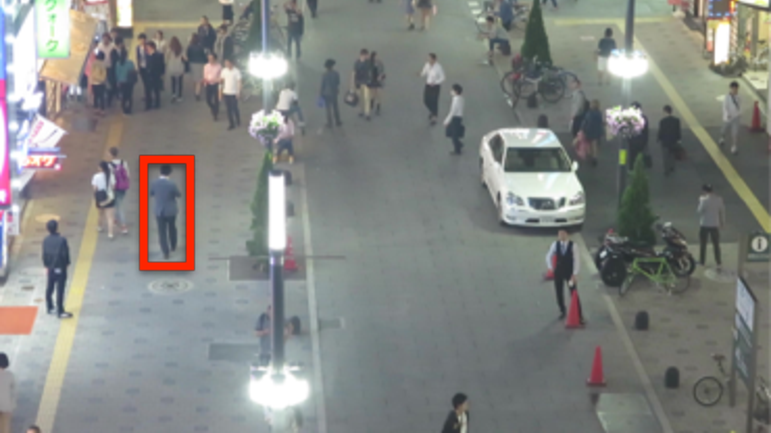
\includegraphics[width=\linewidth]{figures/mot-1.pdf}
      \caption{t=0s, small target in far-field views}
    \end{figure}
    \vspace{-1em}
    \begin{figure}
      \centering
      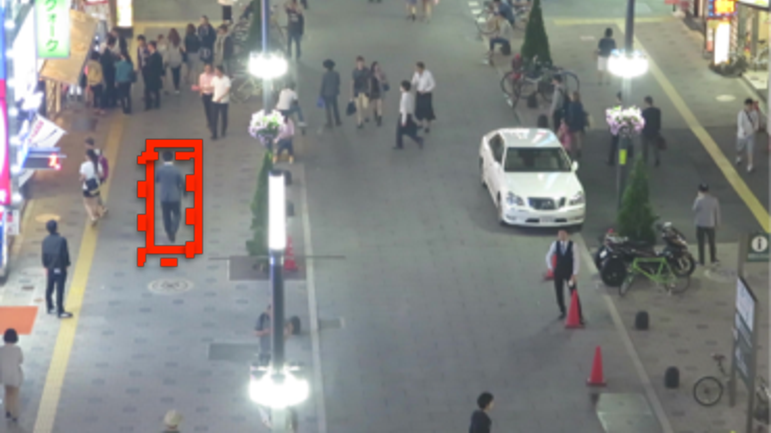
\includegraphics[width=\linewidth]{figures/mot-2.pdf}
      \caption{t=1s, small difference}
    \end{figure}

    \column{0.6\textwidth}
    \vspace{1.5em}

    \begin{tikzpicture}
      \tikzstyle{every node}=[font=\footnotesize]
      \begin{axis}[
        ybar,
        bar width               = .4cm,
        width                   = 1.1\textwidth,
        height                  = 0.4\textheight,
        legend style            = {at = {(0.5, 1.4)}, anchor = north,legend columns = -1},
        symbolic x coords       = {30, 10, 5, 3, 2},
        xtick                   = data,
        enlarge x limits        = 0.15,
        ymin                    = 0,
        ymax                    = 130,
        xlabel                  = {Frame Rate},
        nodes near coords,
        nodes near coords align = {vertical},
        ]
        \addplot table[x=Frame Rate,y=Bandwidth (normalized)]{\stationaryframerate};
        \addplot table[x=Frame Rate,y=Accuracy]{\stationaryframerate};
        \legend{Bandwidth (normalized), Accuracy}
      \end{axis}
    \end{tikzpicture}

    \vspace{1em}

    \begin{tikzpicture}
      \tikzstyle{every node}=[font=\footnotesize]
      \begin{axis}[
        ybar,
        bar width               = .4cm,
        width                   = 1.1\textwidth,
        height                  = 0.4\textheight,
        symbolic x coords       = {1080p, 900p, 720p, 540p, 360p},
        xtick                   = data,
        enlarge x limits        = 0.15,
        nodes near coords,
        nodes near coords align = {vertical},
        ymin                    = 0,
        ymax                    = 130,
        xlabel                  = {Resolution},
        ]
        \addplot table[x = Resolution, y = Bandwidth (normalized)]{\stationaryresolution};
        \addplot table[x = Resolution, y = Accuracy]{\stationaryresolution};
        \legend{}
      \end{axis}
    \end{tikzpicture}
  \end{columns}
\end{frame}


\begin{frame}{Application-specific Optimizations Don't Generalize}
  \captionsetup[figure]{labelformat=empty,font=scriptsize,labelfont=scriptsize}

  \pgfplotstableread[row sep=\\,col sep=&]{
    Frame Rate & Bandwidth (normalized) & Accuracy \\
    30 & 100 & 100 \\
    10 & 65 & 64 \\
    5 & 46 & 32 \\
    3 & 34 & 18 \\
    2 & 27 & 10 \\
  }\mobileframerate
  \pgfplotstableread[row sep=\\,col sep=&]{
    Resolution & Bandwidth (normalized) & Accuracy \\
    1080p & 100 & 100 \\
    900p & 69 & 99 \\
    720p & 49 & 97 \\
    540p & 33 & 93 \\
    360p & 22 & 87 \\
  }\mobileresolution

  \begin{columns}[c]
    \column{0.4\textwidth}
    \vspace{2em}
    \begin{figure}
      \centering
      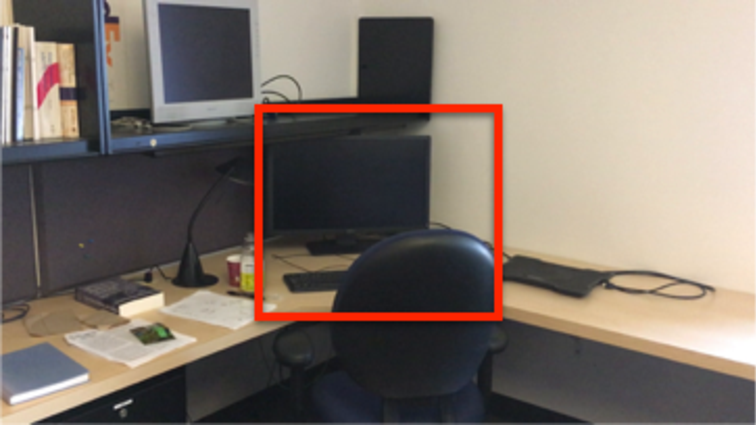
\includegraphics[width=\linewidth]{figures/darknet-1.pdf}
      \caption{t=0s, nearby and large targets}
    \end{figure}
    \vspace{-1em}
    \begin{figure}
      \centering
      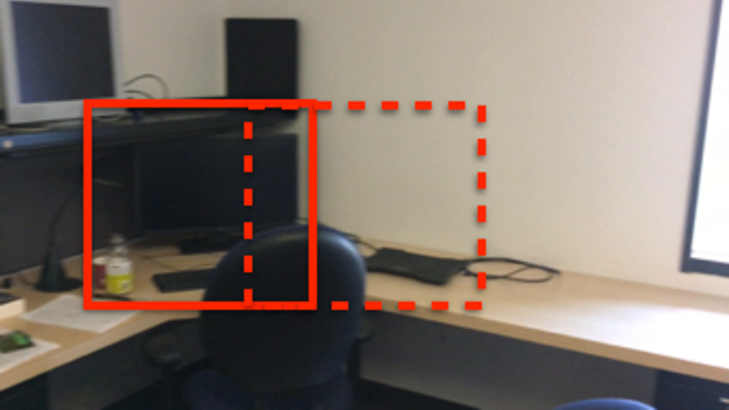
\includegraphics[width=\linewidth]{figures/darknet-2.pdf}
      \caption{t=1s, large difference}
    \end{figure}

    \column{0.6\textwidth}
    \vspace{1.5em}

    \begin{tikzpicture}
      \tikzstyle{every node}=[font=\footnotesize]
      \begin{axis}[
        ybar,
        bar width               = .4cm,
        width                   = 1.1\textwidth,
        height                  = 0.4\textheight,
        legend style            = {at = {(0.5, 1.4)}, anchor = north,legend columns = -1},
        symbolic x coords       = {30, 10, 5, 3, 2},
        xtick                   = data,
        enlarge x limits        = 0.15,
        ymin                    = 0,
        ymax                    = 130,
        xlabel                  = {Frame Rate},
        nodes near coords,
        nodes near coords align = {vertical},
        ]
        \addplot table[x=Frame Rate,y=Bandwidth (normalized)]{\mobileframerate};
        \addplot table[x=Frame Rate,y=Accuracy]{\mobileframerate};
        \legend{Bandwidth (normalized), Accuracy}
      \end{axis}
    \end{tikzpicture}

    \vspace{1em}

    \begin{tikzpicture}
      \tikzstyle{every node}=[font=\footnotesize]
      \begin{axis}[
        ybar,
        bar width               = .4cm,
        width                   = 1.1\textwidth,
        height                  = 0.4\textheight,
        symbolic x coords       = {1080p, 900p, 720p, 540p, 360p},
        xtick                   = data,
        enlarge x limits        = 0.15,
        nodes near coords,
        nodes near coords align = {vertical},
        ymin                    = 0,
        ymax                    = 130,
        xlabel                  = {Resolution},
        ]
        \addplot table[x = Resolution, y = Bandwidth (normalized)]{\mobileresolution};
        \addplot table[x = Resolution, y = Accuracy]{\mobileresolution};
        \legend{}
      \end{axis}
    \end{tikzpicture}
  \end{columns}
\end{frame}

%%% Local Variables:
%%% mode: latex
%%% TeX-master: "../talk"
%%% End:


\begin{frame}{Bandwidth-Accuracy Tradeoff}
  \begin{figure}
    \centering
    \includegraphics[width=0.85\linewidth]{figures/motiv-app-specific.pdf}
    \caption{The measured bandwidth and application accuracy for two video
      analytics applications. (1) Manual policies lack precision without
      measurements and need to handle multiple dimensions (as in a-d). (2)
      Application-specific optimizations do not generalize: degrading frame rates
      works well for stationary camera (a), but not for mobile camera (c). (e-h)
      shows example frames.}
    \label{fig:app-specific}
  \end{figure}
\end{frame}

\begin{frame}{API}
  \begin{table}
    \scriptsize
    \begin{tabular}{ c r l }
      \toprule
      \multirow{4}{*}{Normal}
      & \textit{map} (f: I $\Rightarrow$ O) & Stream<I> $\Rightarrow$ Stream<O> \\
      & \textit{skip} (i: Integer) & Stream<I> $\Rightarrow$
                                     Stream<I> \\
      & \textit{window} (count: Integer, f: Vec<I> $\Rightarrow$ O) & Stream<I> $\Rightarrow$
                                                                      Stream<O> \\
      & ... & ... \\
      \midrule
      \multirow{5}{*}{Degradation}
      & \textit{maybe} (knobs: Vec<T>, f:  (T, I) $\Rightarrow$ I) & Stream<I> $\Rightarrow$
                                                                     Stream<I> \\
      & \textit{maybe\_skip} (knobs: Vec<Integer>) & Stream<I> $\Rightarrow$ Stream<I> \\
      & \textit{maybe\_head} (knobs: Vec<Integer>) & Stream<Vec<I>{}> $\Rightarrow$
                                                     Stream<Vec<I>{}> \\
      & ... & ... \\
      \bottomrule
    \end{tabular}
  \end{table}
\end{frame}

\begin{frame}[fragile]{\texttt{maybe(knobs: Vec<T>, f: (T, I) => I)}}
  \begin{lstlisting}
let quantized_stream = vec![1, 2, 3, 4].into_stream()
    .maybe(vec![2, 4], |k, val| val.wrapping_div(k))
    .collect();
  \end{lstlisting}
  Output: [1, 2, 3, 4] (no degradation), [0, 1, 1, 2] (k=2), or [0, 0, 0, 1]
  (k=4).

  \pause
  \vspace{2em}
  \begin{lstlisting}
let app = Camera::new((1920, 1080), 30)
    .maybe_downsample(vec![(1600, 900), (1280, 720)])
    .maybe_skip(vec![2, 5])
    .map(|frame| frame.show())
    .compose();
  \end{lstlisting}

\end{frame}

\begin{frame}{Applications}
  \begin{table}
    \footnotesize
    \centering
    \begin{tabular}{c c c c}
      \toprule
      Application & Knobs & Accuracy & Dataset \\
      \midrule
      \specialcell{Augmented\\Reality}
                  & \specialcell{resolution \\ frame rate \\ quantization }
                  & F1 score~\cite{Rijsbergen:1979:IR:539927}
                          & \specialcell{iPhone video clips\\training: office (24
      s)\\testing: home (246 s)} \\
      \midrule
      \specialcell{Pedestrian\\Detection}
                  & \specialcell{resolution \\ frame rate \\ quantization }
                  & F1 score
                          & \specialcell{MOT16~\cite{milan2016mot16}\\training: MOT16-04\\testing: MOT16-03} \\
      \midrule
      \specialcell{Log Analysis\\(Top-K, K=50)}
                  & \specialcell{head (N) \\ threshold (T) }
                  & \specialcell{Kendall's $\tau$~\cite{abdi2007kendall}}
                          & \specialcell{\href{https://www.sec.gov}{SEC.gov} logs~\cite{edgarlog} \\ training: 4 days \\
      testing: 16 days} \\
      \bottomrule
    \end{tabular}
    \vspace{0.5em}
    \caption{Application details.}
    \label{tab:apps}
    \vspace{-1em}
  \end{table}
\end{frame}

\begin{frame}{Runtime Adaptation}
  \begin{figure}
    \centering
    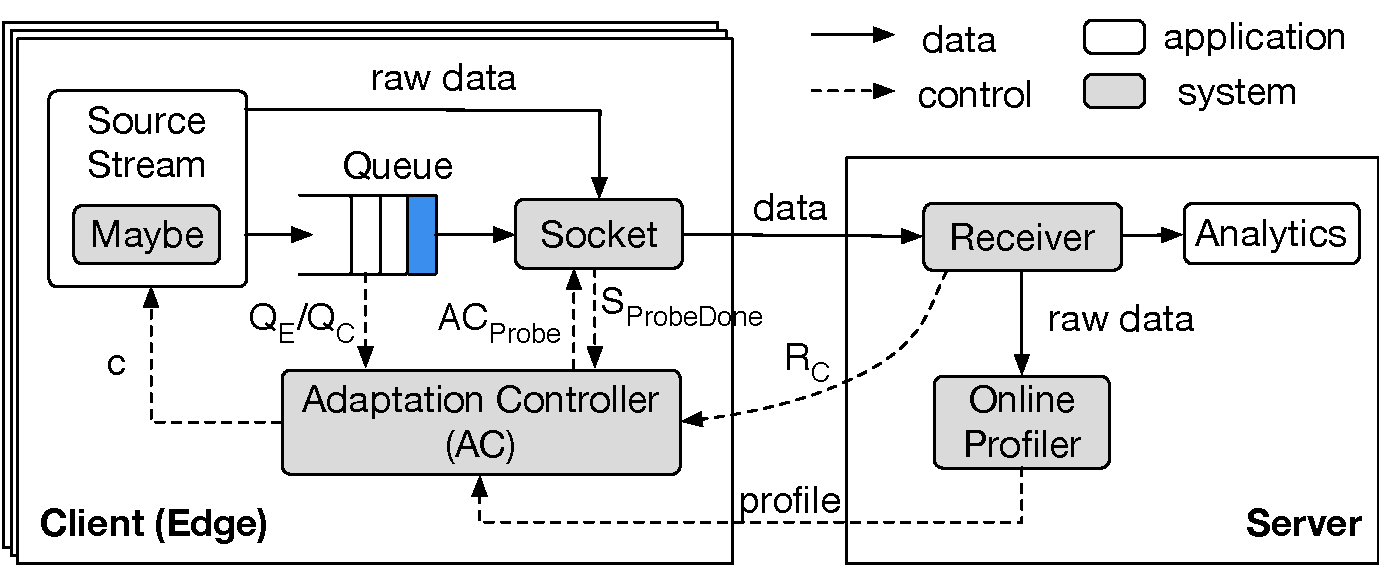
\includegraphics[width=\linewidth]{figures/runtime-adaptation.pdf}
    \caption{Runtime adaptation system architecture.}
    \label{fig:runtime}
  \end{figure}
\end{frame}

\begin{frame}{Top-K}
  \begin{figure}
    \centering
    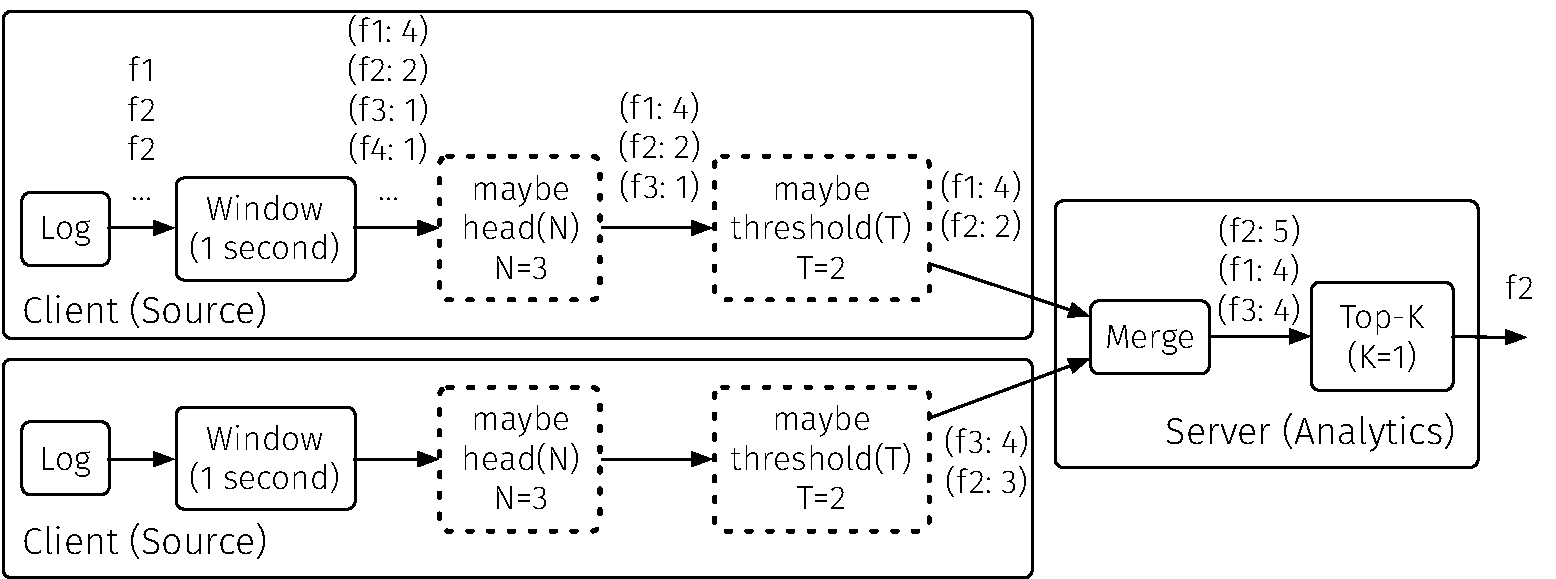
\includegraphics[width=\columnwidth]{figures/topk.pdf}
    \caption{A distributed Top-K application with two degradation operations:
      \texttt{head} and \texttt{threshold}. In this example, \texttt{f2}, which
      is not in Top-1 for either client, becomes the global Top-1 after the
      merge. It would have been purged if the clients use threshold T=3,
      demonstrating degradation that reduces data sizes affects fidelity.}
    \label{fig:topk}
    \vspace{-0.5em}
  \end{figure}
\end{frame}

\begin{frame}{Profiles}
  \begin{figure}
    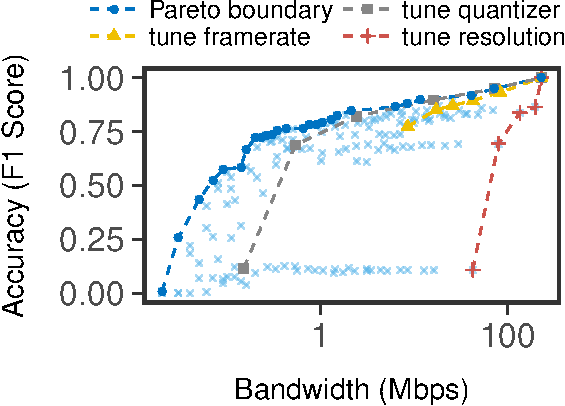
\includegraphics[width=\linewidth]{figures/profile-mot.pdf}
  \end{figure}
\end{frame}


\begin{frame}{All Profiles}
  \begin{figure}[htb]
    \centering
    \begin{subfigure}[t]{0.49\textwidth}
      \centering
      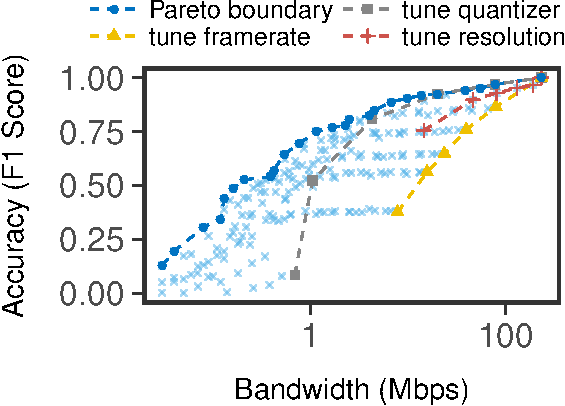
\includegraphics[width=\textwidth]{figures/profile-darknet.pdf}
      \caption{Augmented Reality (AR)}
      \label{fig:ar-profile}
    \end{subfigure}
    \hfill
    \begin{subfigure}[t]{0.49\textwidth}
      \centering
      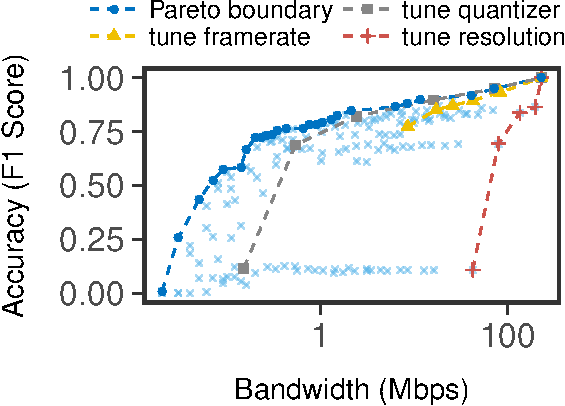
\includegraphics[width=\textwidth]{figures/profile-mot.pdf}
      \caption{Pedestrian Detection (PD)}
      \label{fig:pd-profile}
    \end{subfigure}
    \caption{Application profiles of three applications. Each cross point is one
      configuration $c$'s performance $(B(c), A(c))$. All figures show the
      Pareto boundary as well as the performance if only tuning one
      dimension. Note the x-axis is in log scale.}
    \label{fig:all-profiles}
  \end{figure}
\end{frame}

\begin{frame}{All Profiles}
  \begin{figure}
    \includegraphics[width=0.9\linewidth]{figures/runtime_darknet-timeseries.pdf}
  \end{figure}
\end{frame}

%%% Local Variables:
%%% mode: latex
%%% TeX-master: "talk"
%%% TeX-engine: xetex
%%% End:
